\chapter{Estado del Arte}

\section{Técnicas para el aprendizaje colaborativo}

\subsection{Jigsaw}
Jigsaw es una técnica de aprendizaje colaborativo y recientemente ha sido aplicada por \citeA{Buhr2014429} a un grupo de estudiantes de medicina  de la Universidad de Duke tal y como se describe en el artículo \emph{``Using the Jigsaw Cooperative Learning Method to Teach Medical Students About Long Term and Postacute Care''}. En este estudio se desarrolló una experiencia colaborativa usando la técnica de Jigsaw para exponer a los estudiantes sobre el cuidado intensivo a largo plazo  (LTPAC - Long Term and Post Acute Care) y así lograr que ellos conozcan las herramientas y roles del personal involucrado en este tipo de cuidados de pacientes en un asilo de ancianos. Para alcanzar este objetivo, pequeños grupos de estudiantes de medicina realizaron entrevistas al personal de LTPAC sobre sus respectivos roles. Estos grupos posteriormente fueron reorganizados en nuevos grupos conteniendo un estudiante de cada grupo original más un moderador y cada estudiante en los nuevos grupos tuvo que explicar sobre el rol del profesional LTPAC al cual había entrevistado \cite{Buhr2014429}.\\

Los objetivos del ejercicio jigsaw realizado fueron para definir LTPAC, identificar cuáles son los alcances de este tipo de servicios que se brindan a los pacientes y describir los roles de los miembros del equipo que laboraba en el asilo de ancianos. Para esto, 10 miembros claves del equipo LTPAC fueron identificados y un total de 50 estudiantes fueron divididos en 10 grupos expertos. A cada grupo experto le fue asignado de 30 a 45 minutos para encontrar y entrevistar a 1 miembro del equipo LTPAC(Ver figura \ref{fig:jigsaw_ltpac_1}). Cada estudiante en el grupo tenía que convertirse en un experto sobre el rol del miembro que le fue asignado. Después de las entrevistas, los estudiantes tuvieron un tiempo de 15 minutos para debatir en sus grupos de expertos sobre los aspectos más resaltantes del rol del profesional al que entrevistaron. Finalmente, los grupos fueron reorganizados conteniendo un estudiante experto de cada grupo original así como un moderador(Ver figura \ref{fig:jigsaw_ltpac_2}). Lo nuevos grupos Jigsaw se reunieron por 1 hora durante la cual cada estudiante expuso los resultados de la entrevista que había realizado al profesional LTPAC del asilo \cite{Buhr2014429}.\\



\begin{figure}[h]
  \centering
  % Requires \usepackage{graphicx}
  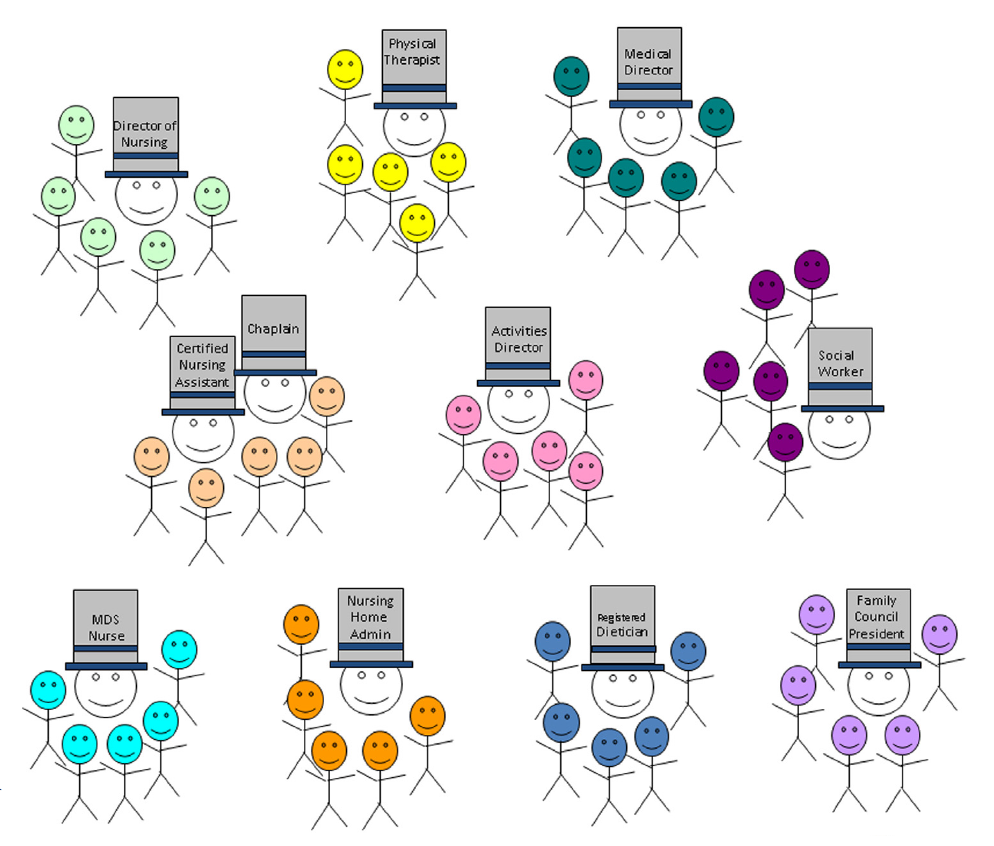
\includegraphics[scale=0.5]{figuras/jigsaw_ltpac_1.png}\\
  \caption[Jigsaw Paso 1]{Jigsaw Primera Fase\protect\cite{Buhr2014429} }
  \label{fig:jigsaw_ltpac_1}
\end{figure}

\begin{figure}[h]
  \centering
  % Requires \usepackage{graphicx}
  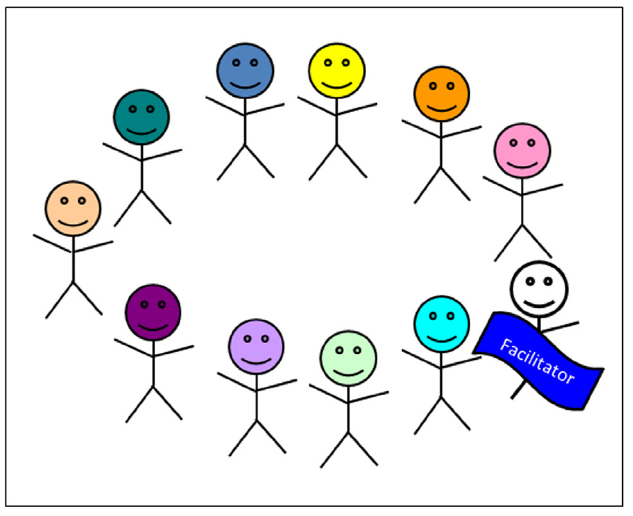
\includegraphics[scale=0.5]{figuras/jigsaw_ltpac_2.png}\\
  \caption[Jigsaw Paso 2]{Jigsaw Segunda Fase\protect\cite{Buhr2014429} }
  \label{fig:jigsaw_ltpac_2}
\end{figure}

La efectividad de esta experiencia de aprendizaje fue medida a través de los comentarios por escrito de los estudiantes y el personal LTPAC así como también a través de una encuesta con una escala de 5 puntos donde 1 reflejaba malo y 5 significaba bueno. Los estudiantes también fueron evaluados con un examen de conocimientos sobre el tema tratado en la actividad desarrollada en el asilo. Los resultados de este examen indicaron que los estudiantes aprendieron los roles del personal LTPAC de forma satisfactoria. En general, el ejercicio jigsaw fue bien recibido por todos los participantes y mostró ser un medio eficaz para introducir a los estudiantes de medicina en el mundo del cuidado de ancianos \cite{Buhr2014429}.\\

\subsection{Pair Research}
En el estudio \emph{``Pair Research: Matching People for Colaboration, Learning, and Productivity''} elaborado por \citeA{miller_pair_2014} se describe una nueva forma de interacción denominada \emph{``Pair Research (Investigación en pares)''} que permite incrementar la productividad, el aprendizaje y la colaboración entre los diferentes grupos de investigación. A lo largo del artículo, los autores detallan un forma de cómo elaborar los grupos y además presentan los resultados obtenidos, los cuales mostraron que los miembros de los equipos usaban la investigación en pares en diferentes maneras incluyendo programación en pares, lluvia de ideas, recolección de data y análisis.\\

Pair Research es una generalización de la programación en pares. Cada semana, los miembros de los grupos son emparejados guidados por algoritmo de emparejamiento. Cada pareja se reune por una a dos horas de las cuales la mitad del tiempo es dedicado a trabajar en el proyecto de la otra persona. El trabajo puede ser cualquier actividad relacionada a programación, pruebas, diseño, recolección de datos y análisis, lluvia de ideas y asesoría. La siguiente semana, se forman nuevas parejas y el proceso se repite.\\

\citeA{miller_pair_2014} elaboraron un prototipo de hoja de cálculo para gestionar la investigación en pares de tal forma que cada semana, el sistema automáticamente hacía recordar a los miembros del grupo que envíen en qué necesitaban ayuda y en qué aspecto cada uno podía ayudar al resto para luego realizar el respectivo emparejamiento y notificar a cada miembro quien sería su siguiente pareja. Lo principal del prototipo elaborado (Ver figura \ref{fig:pair_research}) es la matriz de preferencias para el emparejamiento de personas. Cada semana, los miembros de cada grupo especificaban la ayuda que necesitaban en esa semana como por ejemplo: ``depurar programa en Django'' o ``revisar un informe''. Otros miembros luego completaban la matriz de preferencias de acuerdo a si podían o estaban interesados en ayudar en algún tema en específico; Para esto, ellos tenía que colocar un número según si preferencia siendo 1 el número que refleja mayor interés, -1 el mayor desinterés y 0 indicaba neutro \cite{miller_pair_2014} \\

%\begin{landscape}
\begin{figure}[h]
  \centering
  % Requires \usepackage{graphicx}
  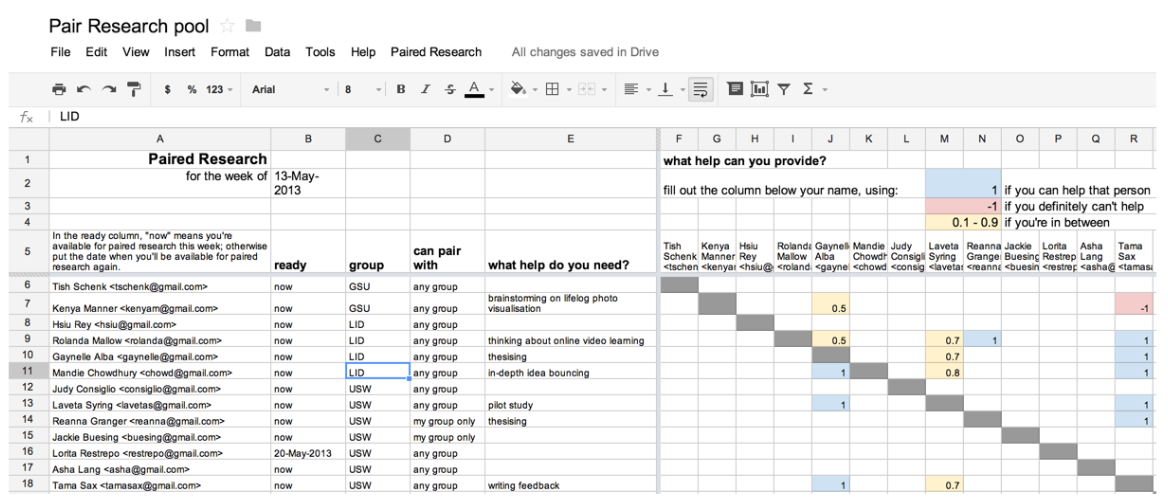
\includegraphics[scale=0.4]{figuras/pair_research.png}\\
  \caption[Pair Research]{Pair research \protect\cite{miller_pair_2014}}
  \label{fig:pair_research}
\end{figure}
%\end{landscape}

La matriz de preferencias sirve para influir en la asignación de parejas de tal forma que aquellos con preferencia mutua positiva sean siempre emparejados mientras que aquellos con preferencia mutua negativa nunca sean emparejados y además se empareje de forma aleatoria a los miembros con preferencia mutua neutral. Para generar las vinculaciones, el sistema utiliza las preferencias ingresadas para formar un grafo ponderado cuyos nodos representan a los miembros del grupo y el grafo contiene un arco entre dos nodos si y solamente si ambos miembros tienen preferencias no negativas. El peso de una arista entre dos miembros es el promedio de sus preferencias mutuas más un plus siempre que ambos miembros no hayan sido emparejados recientemente. Por otro lado, para el caso de aquellos miembros con preferencias neutrales, el sistema agrega una perturbación aleatoria para hacer la asignación entre dichos miembros del grupo \cite{miller_pair_2014}.\\

La finalidad de la investigación en parejas o investigación en pares fue mejorar la productividad, el aprendizaje informal y la colaboración. En cuanto a la productividad, los resultados del estudio mostraron que los miembros se sintieron más motivados al trabajar usando esta técnica y realizaron satisfactoriamente sus trabajos asignados. Respecto al aprendizaje, se observó mejoras sobre herramientas específicas, habilidades, trabajos prácticos, aprendizaje sobre los demás miembros de grupo. Finalmente, en cuanto a colaboración, los integrantes de los grupos lograron interactuar con más personas de lo que usualmente lo harían lo cual incrementó sus oportunidades para colaboraciones futuras \cite{miller_pair_2014}.\\

\newpage
\subsection{Análisis comparativo}
En el siguiente cuadro ser resumen las características principales que nos ofrece cada una de las dos técnicas de aprendizaje colaborativo que han sido presentadas en los apartados anteriores.\\
\begin{longtable}{|L{8cm}|C{2.5cm}|C{2.5cm}|}
\caption{Técnicas de aprendizaje colaborativo}
\label{tab:tecnicasAC}\\
  \hline
  % after \\: \hline or \cline{col1-col2} \cline{col3-col4} ...
  CARACTERÍSTICAS & JIGSAW & PAIR RESEARCH \\
  \hline
  $\diamond$ Se aprende del compañero & \cmark & \cmark\\
  $\diamond$ Permite las revisiones de trabajo constantes & \xmark & \cmark\\
  $\diamond$ Desarrolla la creatividad & \cmark & \cmark\\
  $\diamond$ Mejora las comunicación del estudiante & \cmark & \cmark\\
  $\diamond$ Favorece la integración del grupo	& \cmark & \xmark\\
  $\diamond$ Favorece el aprendizaje del tema a tratar & \cmark & \cmark\\
  $\diamond$ Existe un método para generar los emparejamientos & \xmark & \cmark\\
  $\diamond$ Se requiere la dirección de un profesor &	\cmark & \xmark	\\
  $\diamond$ Permite evitar conflictos interpersonales & \xmark &	\cmark\\
  $\diamond$ Favorece al trabajo con personas conocidas & \cmark & \cmark\\
  $\diamond$ Favorece la integración con nuevas personas &	\cmark & \xmark \\	
  $\diamond$ El alumno elige con quién trabajar & \xmark & \cmark\\		
  \hline
\end{longtable}

\newpage
\section{Herramientas para el aprendizaje colaborativo}

\subsection{LearnCS}
\emph{LearnCS!} es un entorno de programación creado específicamente para el uso de estudiantes de primer año de la carrera de ciencias de la computación. Este programa elimina la necesidad de los alumnos de tener que preocuparse por un editor de texto, comandos linux y proceso de compilación. LearnCS! proveee un entorno web en el cual los alumno pueden escribir, ejecutar y depurar programas usando un interfaz familiar y amigable. El compilador de C embebido que posee el sistema permite al alumno ejecutar sus programas con simplemente hacer click en un botón y obtener los resultados de ejecución de su código fuente \cite{lipman_learncs_2014}.\\

En muchos cursos de programación de primer ciclo, el concepto de depurar un programa es enseñado a finales del curso. En cambio, a través de \emph{LearnCS!}, los alumnos pueden establecer puntos de corte en el programa y empezar a depurar paso a paso su código fuente. Además, el sistema brinda la opción de ver la representación de la memoria y así visualizar en detalle el estado de su programa. Cuando se llaman a funciones, los alumnos aprenden cómo los argumentos y variables locales son colocados en la pila de la memoria y cómo las variables son reservadas en memoria \cite{lipman_learncs_2014}.\\

\begin{figure}[!h]
  \centering
  % Requires \usepackage{graphicx}
  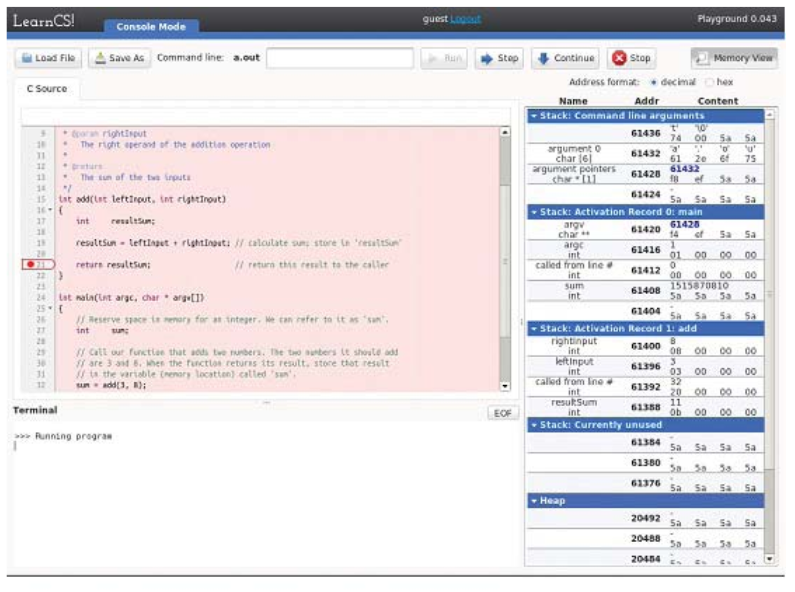
\includegraphics[scale=0.4]{figuras/learncs.png}\\
  \caption[LearnCS]{LearnCS! \protect\cite{lipman_learncs_2014}}
  \label{fig:learncs}
\end{figure}

LearnCS! fue creado para proporcionar un ambiente de aprendizaje para estudiantes de informática de primer año. Sus principales objetivos son proporcionar asistencia útil al alumno en la construcción de un modelo mental de la máquina nocional de C a través de la visualización detallada de la memoria de \emph{LearnCS!} y sus mensajes de error integrados en las instalaciones de depuración, y para proporcionar que producen consejos que son útiles para el principiante para localizar y corregir errores de sintaxis\cite{lipman_learncs_2014}.\\

LearnCS! se ejecuta en un navegador web y tal como se muesta en la Figura \ref{fig:learncs}, ofrece lo siguiente:

\begin{enumerate}
  \item (Panel superior-izquierdo) Un área de la pantalla dedicada a la edición del programa que se está desarrollando.
  \item (Panel derecho) Una representación de la vista de la memoria.
  \item (Panel inferior) Una zona de ``salida'' que contiene una ``terminal'' para la entrada y salida de texto.
  \item (Panel inferior-derecho) Opcionalmente, como se muestra en la figura \ref{fig:learncs2}, se muestra un área gráfica que permite desarrollar programas más interactivos y más interesantes para los alumnos.
\end{enumerate}

\begin{figure}[!h]
  \centering
  % Requires \usepackage{graphicx}
  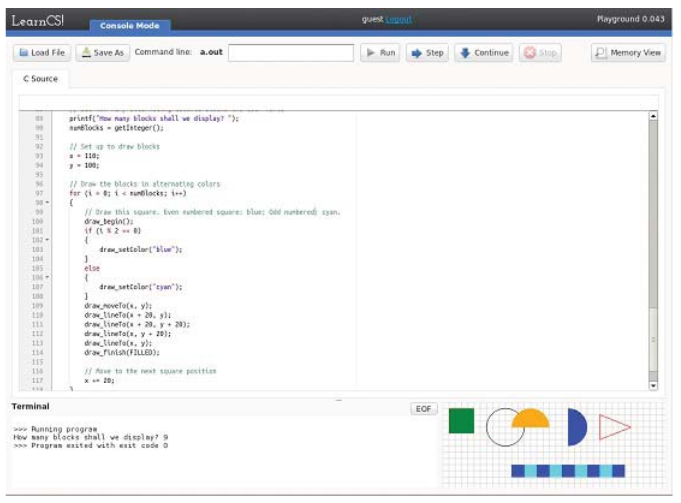
\includegraphics[scale=0.5]{figuras/learncs2.png}\\
  \caption[LearnCS]{LearnCS!}\label{fig:learncs2}
\end{figure}

\newpage
\subsection{Google Docs}

Google Docs es un conjunto de herramientas online que permiten elaborar documentos, hojas de cálculo, dibujos y diapositivas de manera colaborativa usando solamente un navegador web. Esta herramienta es un gestor de documentos pues a través de ella se pueden subir a la nube todo tipo de archivos y ordenarlos en carpetas así como compartirlos con otros usuarios.\\

Para acceder a esta herramienta de colaboración, en primer lugar se debe tener una cuenta de gmail y con ello se obtiene el acceso a Google Docs a través del siguiente link \url{http://docs.google.com/}. Las funcionalidades más resaltantes que posee GoogleDocs son las siguientes:\\

\begin{enumerate}
  \item \emph{Crear documentos básicos desde cero}. Con GoogleDocs es posible realizar tareas que corresponden al manejo de documentos de oficina, como crear documentos de texto, hojas de cálculo, presentaciones de diapositivas, y añadirles a todos ellos imágenes, comentarios o fórmulas, entre otras muchas cosas más.
  \item \emph{Subir archivos ya creados}. Existe la opción de subir archivos que ya están creados y para ellos, Google Docs acepta la mayoría de formatos de archivos comunes como DOC, XLS, ODT, CSV, PPT, PDF, etc.
  \item \emph{Editar un documento}. GoogleDocs posee una barra de herramientas que nos permite aplicar negrita, subrayar, cambiar la fuente, color, etc.
  \item \emph{Compartir documentos.} Cuando se edita un documento, existe la opción de invitar a otros usuarios, enviar el documento por correo electrónico, publicarlo como página web, ver quién tiene acceso, etc.
  \item \emph{Chatear en tiempo real con otros usuarios}.
  \item \emph{Exportar documentos}. Google Docs permite descargar nuestros documentos en el escritorio en archivos Word, Excel, OpenOffice, RTF, PDF, HTML o ZIP.
\end{enumerate}
%A continuación se detalla qué es posible realizar con los documentos, hojas de cálculo y presentaciones que GoogleDocs nos permite elaborar de forma colaborativa.\\

%\textbf{DOCUMENTOS}\\
%
%\begin{itemize}
%  \item Subir documentos de Word, OpenOffice, RTF, HTML o texto (o crear documentos desde cero).
%  \item Invitar a otros usuarios (por su dirección de correo electrónico) para que puedan editar o ver los documentos.
%  \item Editar documentos on line en forma colaborativa con otras personas.
%  \item Ver el historial de revisiones de nuestros documentos y hojas de cálculo y volver a cualquier versión.
%  \item Publicar documentos on line para que estén disponibles para todo el mundo.
%  \item Descargar documentos en el escritorio como documentos de Word, de OpenOffice, RTF, PDF, HTML o ZIP.
%  \item Enviar por correo electrónico los documentos como archivos adjuntos.
%  \item Chatear en tiempo real con otros usuarios.
%\end{itemize}
%
%\textbf{HOJAS DE CÁLCULO}\\
%
%\begin{itemize}
%  \item Importar y exportar datos con los formatos .xls, .csv y .ods
%  \item Usar la edición de formatos y fórmulas en las hojas de cálculo, con lo que podremos calcular resultados y dar a los datos el aspecto que deseemos.
%  \item Chatear en tiempo real con otros usuarios.
%  \item
%  \item
%
%\end{itemize}

\begin{figure}[!h]
  \centering
  % Requires \usepackage{graphicx}
  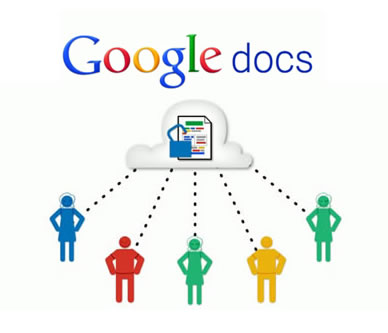
\includegraphics[scale=0.8]{figuras/googledocs.jpg}\\
  \caption[Google Docs]{GoogleDocs \protect\cite{googledocs}}\label{fig:googledocs}
\end{figure}

\newpage
\subsection{Sistema Web para la enseñanza de Casos
de Uso empleando la Técnica de Aprendizaje Cooperativo
de Rompecabezas.}

Este sistema es producto de una tesis de grado implementada en la Pontificia Universidad Católica del Perú. El sistema pretende dar soporte a las tres fases que comprende una clase en la cual se emplea la técnica de Jigsaw para lo cual, se construyeron los módulos de Planificación, Ejecución y Evaluación.\\

El módulo de Planificación permite realizar el diseño de cada sesión de clase. Ahí se plantean los datos de la sesión que serán la base de los objetivos y resultados esperados que permitirán medir el progreso académico de los alumnos.\\

El módulo de Ejecución se encarga de llevar a cabo la ejecución de una sesión de clase basada en la técnica de Jigsaw. Permite el desarrollo paso a paso desde la lectura de materiales, documentos y casos hasta la diagramación de la solución que brinden cada uno de los grupos Jigsaw y Expertos. En este módulo se cuenta con foros de discusión que permiten la comunicación entre los miembros de cada grupo.\\

Por último se tiene el módulo de Evaluación, en el cual se elaboran preguntas y examenes que luego el profesor aplica a sus alumnos. Estos exámenes son calificados manualmente o de forma automática por el propio sistema.

%\subsubsection{ARQUITECTURA DEL SISTEMA}

El sistema fue desarrollado usando una arquitectura Modelo-Vista-Controlador. Se usó Java como plataforma de desarrollo y MySQL como motor de base de datos. Acontinuación se indican los frameworks utilizados en el sistema:

\begin{itemize}
  \item Framework J2EE
  \item Struts 2
  \item MyBatis
  \item Librerías AJAX: JQuery, DojoToolKit
\end{itemize}

El sistema desarrollado consta de 3 módulos que se detallan a continuación:\\

\textbf{Planificación}\\

Este módulo posee las siguientes funcionalidades:
\begin{enumerate}
  \item Crear dinámica de Curso
  \item Consultar información del curso
  \item Consultar configuración de dinámica
  \item Consultar información de dinámica
  \item Actualizar mensaje interno
\end{enumerate}

\textbf{Ejecución}\\

Este módulo se encarga de llevar a cabo el desarrollo de una sesión basada en la técnica de aprendizaje colaborativo de rompecabezas. Permite la lectura de materiales y documentes, hasta la elaboración colaborativa de la solución a los diferentes problemas propuestos en los diferentes grupos Jigsaw y Expertos.\\

El módulo cuenta con herramientas de chat para la comunicación online, así como también de un foro para la discusión de los temas.\\

Este módulo posee las siguientes funcionalidades:

\begin{enumerate}
  \item Actualizar publicación en foro
  \item Ingresar sesión cooperativa
  \item Controlar estado de la dinámica
  \item Elaborar casos de uso,.
\end{enumerate}

\textbf{Evaluación}\\

En esta parte del sistema es donde se elaboran las preguntas y exámenes por parte del docente y posteriormente se aplican a los alumnos. El sistema permite que estos exámenes sean evaluados manualmente o de forma automática.

Este módulo posee las siguientes funcionalidades:
\begin{enumerate}
  \item Consultar configuración de evaluación.
  \item Consultar corrección de evaluación.
  \item Consultar calificación de evaluación.
  \item Crear evaluación.
  \item Rendir evaluación.
  \item Realizar calificación.
\end{enumerate}


\emph{Fuente} \cite{pinzas_desarrollo_2013}

\subsection{CodeBunks}
\begin{figure}[h]
  \centering
  % Requires \usepackage{graphicx}
  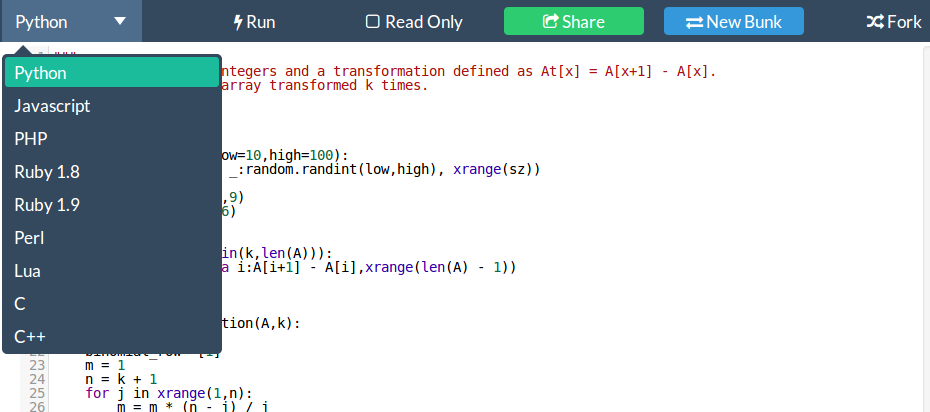
\includegraphics[scale=0.3]{figuras/codebunk.png}\\
  \caption[CodeBunk]{Codebunk \protect\cite{codebunk}}\label{fig:codebunk}
\end{figure}
Es una plataforma que permite codificar y compilar en diferentes lenguajes de programación de forma colaborativa y en tiempo real. Algunas de sus funcionalidades son las siguientes:\\

\begin{enumerate}
  \item Posee un editor colaborativo que soporta 14 lenguajes de programación, tiene coloración de sintaxis según el lenguaje y brinda un indentado inteligente.
  \item Compilar y Ejecutar. La plataforma permite compilar y ejecutar código en Python, Java, C, C++, Ruby, Javascript, entre otros.
  \item Audio y Video Chat.
  \item Code playback. Permite repetir la historia de los cambios realizados en el código.
  \item Equipos. Permite crear equipos de trabajo e invitar a otros usuarios a colaborar en el desarrollo de un programa.
\end{enumerate}


\newpage
\subsection{Análisis comparativo}
Las cuatro herramientas para el aprendizaje colaborativo que se han estudiado hasta el momento son resumidas y comparadas en el siguiente cuadro, en el cual se podrá apreciar las características que nos ofrece cada una de las cuatro aplicaciones presentadas anteriormente.\\
%\begin{landscape}
\begin{longtable}{|L{7cm}|C{1.5cm}|C{1.5cm}|C{1.5cm}|C{1.5cm}|}
\caption{Herramientas para el aprendizaje colaborativo}
\label{tab:herramientasAC}\\
    \hline
    CARACTERÍSTICAS	& LearnCS &	Google Docs & Sistema PUCP & Code Bunks\\	
    \hline
    $\diamond$ Permite escribir código fuente C	&\cmark	&\cmark	&\xmark	&\cmark	\\
    $\diamond$ Compila código fuente C	&\cmark	&\xmark	&\xmark	&\cmark	\\
    $\diamond$ Permite depurar el código fuente C	&\cmark	&\xmark	&\xmark	&\xmark	\\
    $\diamond$ Posee un representación de la memoria del computador	&\cmark	&\xmark	&\xmark	&\xmark	\\
    $\diamond$ Muestra mensajes de error	&\cmark	&\xmark	&\xmark	&\cmark	\\
    %$\diamond$ Brinda coloreado de sintaxis de lenguaje C	&\cmark	&\xmark	&\xmark	&\cmark	\\
    $\diamond$ Es un aplicativo web	&\cmark	&\cmark	&\cmark	&\cmark	\\
    $\diamond$ Soporta sólamente lenguage C	&\cmark	&\xmark	&\xmark	&\xmark	\\
    $\diamond$ Crear documentos básicos desde cero	&\xmark	&\cmark	&\xmark	&\xmark	\\
    $\diamond$ Subir archivos ya creados	&\xmark	&\cmark	&\xmark	&\xmark	\\
    $\diamond$ Edición de documentos de texto	&\xmark	&\cmark	&\cmark	&\cmark	\\
    $\diamond$ Edición de hojas de cálculo	&\xmark	&\cmark	&\xmark	&\xmark	\\
    $\diamond$ Edición de diapositivas	&\xmark	&\cmark	&\xmark	&\xmark	\\
    $\diamond$ Compartir documentos	&\xmark	&\cmark	&\xmark	&\cmark	\\
    $\diamond$ Chatear en tiempo real con otros usuarios	&\xmark	&\cmark	&\xmark	&\cmark	\\
    $\diamond$ Exportar documentos 	&\xmark	&\cmark	&\xmark	&\xmark	\\
    $\diamond$ Diseñar sesión de clase jigsaw	&\xmark	&\xmark	&\cmark	&\xmark	\\
    $\diamond$ Tomar evaluaciones	&\xmark	&\xmark	&\cmark	&\xmark	\\
    $\diamond$ Calificar evaluaciones	&\xmark	&\xmark	&\cmark	&\xmark	\\
    $\diamond$ Foro de discusión	&\xmark	&\xmark	&\cmark	&\xmark	\\
    $\diamond$ Elaborar casos de uso	&\xmark	&\xmark	&\cmark	&\xmark	\\
    $\diamond$ Permite escribir código fuente de forma colaborativa	&\xmark	&\cmark	&\xmark	&\cmark	\\
    $\diamond$ Soporta varios lenguajes de programación (14)	&\xmark	&\xmark	&\xmark	&\cmark	\\
    $\diamond$ Coloración de sintaxis	&\cmark	&\xmark	&\xmark	&\cmark	\\
    $\diamond$ Indentado inteligente	&\xmark	&\xmark	&\xmark	&\cmark	\\
    $\diamond$ Compilador de código fuente	&\xmark	&\xmark	&\xmark	&\cmark	\\
    $\diamond$ Ejecución de código fuente	&\xmark	&\xmark	&\xmark	&\cmark	\\
    $\diamond$ Visualización de resultados de ejecución	&\xmark	&\xmark	&\xmark	&\cmark	\\
    $\diamond$ Historial de revisiones de código	&\xmark	&\cmark	&\xmark	&\cmark	\\
    $\diamond$ Creación de equipos colaborativos	&\xmark	&\cmark	&\xmark	&\cmark	\\
    \hline
\end{longtable}
%\end{landscape}

\newpage
\section{Frameworks para aplicaciones web de tiempo real}

\subsection{GoogleDrive Realtime API}

La API de GoogleDrive en tiempo real ofrece el trabajo colaborativo como un servicio para los archivos en Google Drive a través del uso de las transformaciones operativas. El API es una biblioteca JavaScript que ofrece a los desarrolladores objetos de colaboración, eventos y métodos para la creación de aplicaciones en las cuales se puedan realizar tareas colaborativas.\\

Esta API permite a los desarrolladores diseñar un modelo de datos común que se ve como un modelo local en memoria. Se pueden escribir código para manipular listas, arrays, matrices, maps, y objetos javascript propios del desarrollador. Cada vez que se modifique un modelo de datos, éste automáticamente cambiará para todos los usuarios presentes en el documento.\\

La API está basada en la misma tecnología de colaboración usada por GoogleDocs y por ello, cada vez que un modelo de datos es modificado, el cambio es aplicado inmediatamante a la copia local del documento y luego, la API envía una representación del cambio al servidor de tal forma que el cambio es guardado en el documento y comunicado a los demás colaboradores.\\

La API en tiempo real se encarga de todos los aspectos de la transmisión de datos, el almacenamiento y la resolución de conflictos cuando varios usuarios están editando un archivo. En general, la API nos brinda lo siguiente:

\begin{enumerate}
  \item Funciones para cargar y trabajar documentos en tiempo real.
  \item Objetos construídos colaborativamente(cadenas, listas, y mapas).
  \item La capacidad de crear objetos propios que puedan personalizarse.
  \item Eventos para la detección de cambios en el modelo de colaboración y detección del ingreso o salida de colaboradores.
\end{enumerate}
La API en tiempo real de GoogleDrive proporciona todas las herramientas que se necesitan para crear una aplicación colaborativa que no necesita correr en nuestro propio servidor.


%\subsection{Socket.IO}
%
%Socket.IO permite la comunicación basada en eventos bidireccional en tiempo real.
%Funciona en todas las plataformas, el navegador o dispositivo, centrándose también en la fiabilidad y la velocidad.
%\begin{itemize}
%  \item Análisis en tiempo real
%  \item Transmisión binaria. A partir de 1.0, es posible enviar cualquier tipo de archivo: imagen, audio, video.
%  \item Mensajería instantánea y chat
%  \item Colaboración de documentos. Permitir a los usuarios editar simultáneamente un documento y ver los cambios del otro.
%\end{itemize}

\subsection{Ideone API - Sphere Engine}
Sphere Engine, antes conocida como Ideone API, permite a los usuarios ejecutar código en múltiples lenguajes de manera online. Ideone es un compilador y una herramienta de depuración que soporta más de 60 lenguajes de programación. Através de la API, los desarrolladores pueden crear sus propias aplicaciones con fines educativos, personales o de negocios. Sphere Engine es un servicio web el cual puede ser accedido a través de protocolo SOAP.\\

Esta API posee las siguientes funcionalidades:

\begin{enumerate}
  \item Permite subir código fuente y compartirlo con otros usuarios.
  \item Permite ejecutar el código fuente con una data inicial en el lado servidor y en más de 60 lenguajes de programación diferentes.
  \item Permite descargar los resultados obtenidos en la ejecución del código fuente(salida, errores, información de compilación, tiempo de ejecución, uso de memoria, etc).
\end{enumerate}
\begin{figure}[h]
  \centering
  % Requires \usepackage{graphicx}
  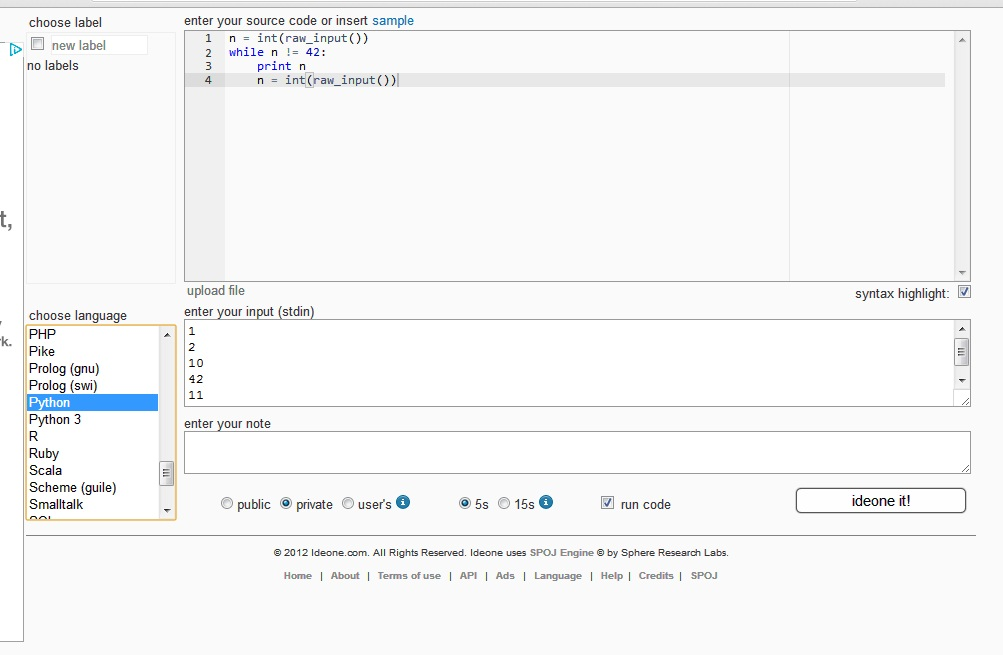
\includegraphics[scale=0.5]{figuras/ideone.jpg}\\
  \caption[Ideone]{Ideone \protect\cite{ideone}}\label{fig:ideone}
\end{figure}


\newpage
\subsection{Análisis comparativo}
Tanto la API de GoogleDrive como la API de Ideone ofrecen características importantes para la elaboración de aplicaciones web de tiempo real, las mismas que se detallan en el siguiente cuadro comparativo.\\
\begin{longtable}{|L{10cm}|C{2cm}|C{2cm}|}
\caption{Frameworks para aplicaciones web de tiempo real}
\label{tab:frameworks}\\
\hline
CARACTERÍSTICAS & Google Drive Realtime API	& Ideone API - Sphere Engine\\	
\hline
$\diamond$ Se implementa a través de Javascript	&\cmark	&\xmark	\\
$\diamond$ Creación y edición de listas, arrays, matrices, maps, objetos javascript personalizados		&\cmark	&\xmark	\\
$\diamond$ Detección de cambios	&\cmark	&\xmark	\\
$\diamond$ Detección de ingreso o salida de colaboradores	&\cmark	&\xmark	\\
$\diamond$ Ejecutar código en múltiples lenguajes de manera online	&\xmark	&\cmark	\\
$\diamond$ Servicio web vía protocolo SOAP	&\xmark	&\cmark	\\
$\diamond$ Permite cargar código fuente	&\xmark	&\cmark	\\
$\diamond$ Permite ejecutar código fuente	&\xmark	&\cmark	\\
$\diamond$ Permite subir data de prueba inicial	&\xmark	&\cmark	\\
$\diamond$ Permite descargar los resultados obtenidos en la ejecución	&\xmark	&\cmark	\\
\hline
\end{longtable}

